\documentclass[12pt, a4paper]{article}
\usepackage{amsmath}
\usepackage{amsfonts}
\usepackage{amsthm}
\usepackage{mathtools}
\newtheorem{theorem}{Theorem}[section]
\newtheorem{definition}{Definition}[section]
\numberwithin{equation}{section}
\usepackage{pgfplots}
\pgfplotsset{width=10cm,compat=1.9}
\graphicspath{ {img/} }
\DeclareGraphicsExtensions{.png}

\title{Reinforcement Learning}
\author{Kristian Wichmann}

\begin{document}
\maketitle

\section{Basics of reinforcement learning}
\textit{Reinforcement learning} deals with an \textit{agent} making \textit{decisions} over time in dealing with some \textit{environment}, to maximize some cumulative, scalar \textit{reward}.

An example would be playing a video game. Here, the player is the agent. The control inputs are the decisions. The game and its internal logic is the environment. And the score is the reward.

Sometimes, a reward will be greater if it is postponed - it is not always advantagegous to reap any immediate reward. In other words, reinforcement learning algorithms will not benefit from being greedy.

\subsection{The reward hypothesis}
The basis of all reinforcement learning is the \textit{reward hypothesis}, which states:

\begin{quotation}
All goals can be described by the maximization of some cumulative, expected reward.
\end{quotation}

\subsection{Observation, action, and reward}
At at given timestep $t$, a reinforcement learning agent gets some input; an \textit{observation} $O_t$ about the environment. It then takes an \textit{action} $A_t$. And finally it gets a scalar \textit{reward} $R_t$.

\begin{figure}
\centering
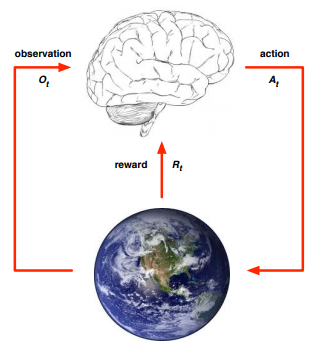
\includegraphics[width=0.6\textwidth]{agent_environment}
\caption{The interplay between agent and environment.}
\label{fig:agent_environment}
\end{figure}

\subsection{History and state}
At any given time step $t$, the agent has a \textit{history} $H_t$, which simply consist of all the observations, actions, and rewards that have happened so far:
\begin{equation}
H_t=O_1,A_1,R_1,O_2,A_2,R_2,\cdots,O_t,A_t,R_t,
\end{equation}
A \textit{state} is a way for to parse this history into a more meaningful form. Formally, the state representation is simply a function of the history:
\begin{equation}
S_t=f(H_t)
\end{equation}

It is very important to note, that this is generally distinct from the \textit{environment state} $H^e_t$. The environment state contains complete information about the environment, including data and mechanisms that may be hidden to the agent. Hence $H^e_t$ can depend on other things than just the history. Such information is \textit{private} to the environment.

The \textit{agent state} $S^a_t$ on the other hand is the internal representation the agent uses to decide on which actions to take. Once again, it can be any function of history:
\begin{equation}
S^a_t=f(H_t)
\end{equation}

\subsection{Markov states}
A state $S_{t+1}$ is called a \textit{Markov state} or an \textit{information state} if it only depends on the state of the previous time step. Expressed probabilistically:
\begin{equation}
\mathbb{P}[S_{t+1}|S_1,S_2,\cdots S_t]=\mathbb{P}[S_{t+1}|S_t]
\end{equation}
In other words, we don't need the entire history to decide on an action: Knowing the present is enough. Or put another way:
\begin{quotation}
The future is independent of the past, given the present.
\end{quotation}
Or:
\begin{quotation}
The state is a \textit{sufficient statistic} of the future.
\end{quotation}

The environment state is always Markov, as by definition it contains all information about what can happen next. Similarly, the state consisting of the entire history is trivially Markov as well.

\subsection{Full observability}
This is the case where, in fact, we can observe everything about the environment and its inner workings. So that:
\begin{equation}
O_t=S^a_t=S^e_t
\end{equation}
Sometimes this is reasonable. Sometimes not. But it will be a useful theoretical situation. This is known as a \textit{Markov decision process} or MDP for short.

When this condition is not fulfilled, we speak about \textit{partial observability} or a \textit{partially observable evironment}. Here the agent only indirectly observes the invironment. This situation is known as a \textit{partially observable Markov decision process} or POMDP for short.

\subsection{State example: Bayesian beliefs}
This state representation can be seen as a current best bet at what the actual environment state is. In other words, it is represented by Bayesian probabilities, which may then be updated over time using Bayes' rule:
\begin{equation}
S^a_t=(\mathbb{P}[S^e_t=s_1],\mathbb{P}[S^e_t=s_2],\cdots,\mathbb{P}[S^e_t=s_n])
\end{equation}

\subsection{State example: Recurrent neural net}
Here, the state $S^a_t$ is a linear combination of the observation $O_t$ and the state of the last time step $S^a_{t-1}$, followed by a non-linear \textit{activation function} $\sigma$:
\begin{equation}
S^a_t=\sigma(W_O O_t+W_S S^a_{t-1})
\end{equation}
Here, the $W$'s are weight matrices with sizes corresponding to the dimenstionality of observations and state vectors. Typical choices for $\sigma$ are sigmoid, tanh, or rectified linear unit.

\section{Components of an agent}
A reinforcement learning agent may contain one or more of the following components:
\begin{itemize}
\item \textit{Policy}: The agent's behaviour function. Shows how the agent gets from its state to deciding on an action.
\item \textit{Value function}: A measure of how desirable it is to be in a given state, or perform a given action.
\item \textit{Model}: The agent's representation of the environment.
\end{itemize}
We'll examine each of these in greater detail below:

\subsection{Policy}
A policy $\pi$ is a mapping from state to action. For a \textit{deterministic} policy, this is an ordinary function:
\begin{equation}
\pi(s)=a
\end{equation}
So the state $s$ is always mapped to the action $a$. We should ideal choose $\pi$ so that the reward is maximized. 

But a policy can also be \textit{stochastic}, i.e. probabilistic. In this case $\pi$ takes the form of conditional probabilities:
\begin{equation}
\pi(a|s)=\mathbb{P}[A=a|S=s]
\end{equation}

\subsection{Value function}
A value function $V_\pi$ is a prediction of the future reward for state $s$ under a given policy $\pi$:
\begin{equation}
V_\pi(s)=\mathbb{E}_\pi[R_t+\gamma R_{t+1}+\gamma^2 R_{t+2}+\cdots|S_t=s]
\end{equation}
Here $\gamma$ is a \textit{discounting factor}, between 0 and 1. 0 means that we only care about the immediate reward, while values approaching 1 means that we care progressively more about long run rewards.

\subsection{Model}
In this context, a model tries to predict the evolution of the environment. These can take two different forms:
\begin{itemize}
\item \textit{Transition prediction} $\mathcal{P}$ models the change of state of the environment:
\begin{equation}
\mathcal{P}^a_{ss'}=\mathbb{E}[S_{t+1}=s'|S_t=s, A_t=a]
\end{equation}
\item \textit{Reward prediction} $\mathcal{R}$ models the change in (immediate) reward:
\begin{equation}
\mathcal{R}^a_s=\mathbb{E}[R_{t+1}|S_t=s, A_t=a]
\end{equation}
\end{itemize}

\begin{figure}
\centering
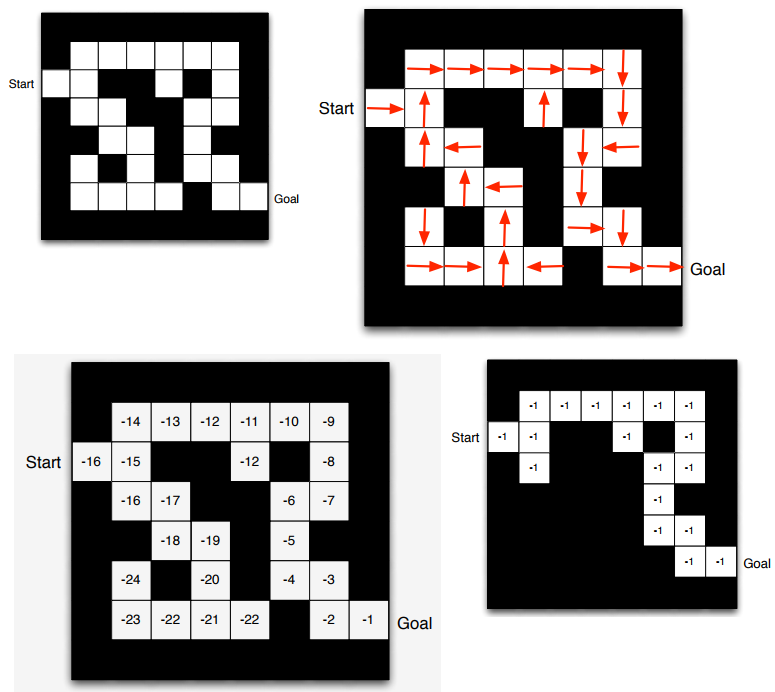
\includegraphics[width=\textwidth]{maze}
\caption{Upper left: Maze example. Upper right: Policy for maze. Lower left: Value function for maze. Lower right: Reward prediction for maze.}
\label{fig:maze}
\end{figure}

\subsection{Example: Maze}
As an example, consider an agent that has to find its way though the maze in the upper left of figure \ref{fig:maze}.  The problem has the following qualities:
\begin{itemize}
\item Rewards: We want the agent to get through the maze as quickly as possible, so each time step has a reward of -1.
\item Actions: The agent can move up, down, left, or right in each time step.
\item State: The state is the agents current position square in the maze.
\end{itemize}

A good policy for solving the problem is shown in the upper right. Here the arrows dictates the action given the state (position).

The lower left shows the value function corresponding to the policy: The future reward is negative the number of steps needed to get out of the maze from the current state (position). An optimal action can be chosen greedily, by picking the possibility with the lowest value of the function.

The lower right shows a reward prediction model for the maze. This one technically depends on both state and action, but as we no it is -1 no matter what.

\subsection{Categorization of agents}
Based on the above, we can broadly categorize agents into several categories:
\begin{itemize}
\item\textit{Value based agents} are based on a value function - with the policy being implicit. I.e. in each step we can greedily pick the action with the highest future reward, based directly on the value function.
\item\textit{Policy based agents} on the other hand has the policy as its key ingredient. Here, the policy mapping directly shows what action to take in each state.
\item\textit{Actor critic agents} takes both a poicy and a value function into account. Ideally the "best of both worlds".
\item\textit{Model free agents} may by policy and/or value function based, but has no model! I.e. it doesn't try to make predictions about the environment.
\item\textit{Model agents} may by policy and/or value function based, but includes modelling.
\end{itemize}

\section{Reinforcement learning and planning}
There's two fundamental types of problems in sequential decision making: \textit{Reinforcement learning} and \textit{planning}.

Reinforcement learning can be viewed as dumping the agent into an alien environment it initially knows nothing about. The agent then begins to interact with the environment, eventually improving its policy for doing so.

Planning is the situation where the agent starts with a perfect model of the environment. The agent then uses this model to make calculations without any external interaction, which then informs policy.

So in planning, we can in principle look many steps ahead, determining states and rewards (or expectation values thereof) and use this to pick optimal actions. In other words, a tree search.

\subsection{Exploration versus exploitation}
So reinforcement learning is very much a trial-and-error process. The agent should hopefully learn an effective policy from interacting with the environment. This requires \textit{exploration}. Ideally without losing too much reward along the way.

\begin{quotation}
Exploration finds more information about the environment.
\end{quotation}

Planning, on the other hand relies on \textit{exploitation} of the complete knowledge of the environment.

\begin{quotation}
Exploitation uses known information to maximize reward.
\end{quotation}

Usually, a combination of exploration and exploitation is necessary for achieving success. So there's a balance between the two, sometimes knows as \textit{exploration-exploitation tradeoff}. This consideration is unique to reinforcement learning as opposed to machine learning as a whole.

\subsubsection{Examples}
Situation: You're going out to eat.
\begin{itemize}
\item Exploitation: Going to your favorite restaurant.
\item Exploration: Trying a new restaurant.
\end{itemize}
Situation: Online banner advertisement.
\begin{itemize}
\item Exploitation: Show the most succesful advert so far.
\item Exploration: Display a different advert.
\end{itemize}
Situation: Drilling for oil.
\begin{itemize}
\item Exploitation: Drill at the best known location.
\item Exploration: Drill at a new location.
\end{itemize}

\subsection{Prediction and control}
\textit{Prediction} is trying out a given policy in practice and evaluating the results.

\textit{Control} on the other hand is optimizing the future, i.e. finding the best strategy.

Usually in reinforcement learning, we have to do prediction in order to control.

\section{Markov reward processes}
Recall that a Markov decision process (or MDP for short) is a case where everything about the environment is known - the agent state is the same as the environment state. This also means that it has the Markov property.

It turns out that almost all reinforcement learning problems can be restated as MDP's. For instance:
\begin{itemize}
\item Optimal control primarily deals with continuous MDP's.
\item Partially observable problems can be conversted into MDP's.
\item \textit{Bandits} are MDP's with one state.
\end{itemize}
In this section, we will deal with a simpler case - known as Markov reward processes - and the tackle the general problem later.

\subsection{Transition probability matrix}
Consider for a moment an agent with a state having the Markov property, which simply takes the same (or no) action in every time step. Then given the initial state $s$ there is a probability it will end up in state $s'$ in the next time step - it can depend only on $s$ and $s'$ per the Markov property:
\begin{equation}
\mathcal{P}_{ss'}=\mathbb{P}[S_{t+1}=s'|S_t=s]
\end{equation}
These propabilities form a matrix; the \textit{transition probability matrix} $\mathcal{P}$:
\begin{equation}
\mathcal{P}=\begin{pmatrix}
\mathcal{P}_{11} & \mathcal{P}_{12} & \cdots & \mathcal{P}_{1n}\\
\mathcal{P}_{21} & \mathcal{P}_{22} & \cdots & \mathcal{P}_{2n}\\
\vdots & \vdots & \ddots & \vdots \\
\mathcal{P}_{n1} & \mathcal{P}_{n2} & \cdots & \mathcal{P}_{nn}
\end{pmatrix}
\end{equation}
This form assumes a finite number of states $n$, but in principle this can be infinite.

Because the entries are probabilites, each row of $\mathbb{P}$ must sum to 1:
\begin{equation}
\forall i\in\{1, 2,\ldots,n\}:\ \sum_{j=1}^n\mathcal{P}_{ij}=1
\end{equation}

Such a system - represented by the tuple $\langle S,\mathcal{P}\rangle$ - is known as a \textit{Markov process} or \textit{Markov chain}.

\subsection{Markov reward processes}
A \textit{Markov reward process} (or MRP) is a Markov process with a finite set of states and a \textit{reward function} $\mathcal{R}$ as well as a discount factor $\gamma\in[0,1]$. The reward function is defined as the expectation value of the next reward given the current state:
\begin{equation}
\mathcal{R}: s\mapsto\mathcal{R}_s=\mathbb{E}[R_{t+1}|S_t=s]
\label{reward}
\end{equation}
So a Markov reward process is the tuple $\langle S,\mathcal{P},\mathcal{R},\gamma\rangle$

\subsection{Return and value function}
The \textit{return} of a given outcome of a Markov reward process\footnote{Or of any system with rewards and a discounting factor $\gamma$, really.} is:
\begin{equation}
G_t=R_{t+1}+\gamma R_{t+2}+\gamma^2 R_{t+3}+\cdots=\sum_{n=1}^\infty \gamma^{n-1} R_{t+n}
\label{return}
\end{equation}
In other words, the return is the discounted future reward. This is the quantity we wish to maximize.

The value function, as we've already discussed above, is the expectation value of the return:
\begin{equation}
v(s)=\mathbb{E}[G_t|S_t=s]
\label{value}
\end{equation}

\subsection{The Bellman equation for MRP's}
We can now use equations \ref{value}, \ref{return}, and \ref{reward} to get a recursive formula for the value function:
\begin{align}
v(s)=&\mathbb{E}[G_t|S_t=s]=\\
&\mathbb{E}[R_{t+1}+\gamma R_{t+2}+\gamma^2 R_{t+3}+\cdots|S_t=s]=\\
&\mathbb{E}[R_{t+1}+\gamma(R_{t+2}+\gamma R_{t+3}+\gamma^2 R_{t+4}+\cdots)|S=s]=\\
&\mathbb{E}[R_{t+1}+\gamma G_{t+1}|S_t=s]=\\
&\mathbb{E}[R_{t+1}|S_t=s]+\gamma\mathbb{E}[G_{t+1}|S_t=s]=\\
&\mathcal{R}_s+\gamma\sum_{s'=1}^n\mathbb{P}[G_{t+1}|S_{t+1}=s']\mathbb{P}[S_{t+1}=s']=\\
&\mathcal{R}_s+\gamma\sum_{s'=1}^n\mathcal{P}_{ss'}v(s')
\end{align}
Here, $\mathcal{R}_s$ is the reward for leaving state $s$ - which might seem somewhat backwards. Summing it up:
\begin{equation}
v(s)=\mathcal{R}_s+\gamma\sum_{s'=1}^n\mathcal{P}_{ss'}v(s')
\label{bellman}
\end{equation}
Treating the value and reward functions as vectors $v$ and $\mathcal{R}$, this can be rewritten in matrix form:
\begin{equation}
v=\mathcal{R}+\gamma\mathcal{P}v
\label{belmann_matrix}
\end{equation}
This equation can be solved using the usual methods:
\begin{equation}
v=\mathcal{R}+\gamma\mathcal{P}v\Leftrightarrow(I_n-\gamma\mathcal{P})v=\mathcal{R}\Leftrightarrow v=(I_n-\gamma\mathcal{P})^{-1}\mathcal{R}
\end{equation}
This direct solution however, is only tractable for small $n$, as the run time for matrix inversion is $O(n^3)$. Instead, there is a number of other, faster possibilities, including:
\begin{itemize}
\item Dynamic programming.
\item Monte-Carlo evaluation.
\item Temporal difference learning.
\end{itemize}

\subsubsection{Intuition behind the Bellman equation for MRP's}
What is the intuition behind equation \ref{bellman}? Imagine the agent is in state $s$. We wish to calculate the expectation of the future discounted reward. First we leave $s$ which gives an immediate reward of $\mathcal{R}_s$. To get the future reward we have to make a weighted average over all the possible states we can go to from $s'$, each having a future reward of $v(s')$. Finally this is discounted by multiplying with $\gamma$.

\section{Markov decision processes}
Now for the full MDP treatment. This case is very similar to the MRP case, but now there is several different actions to choose from, collectively written as $\mathcal{A}$. To each action $a\in\mathcal{A}$, corresponds a transition probability matrix $\mathcal{P}^a$. So formally, a Markov decision process is a tuple $\langle\mathcal{S},\mathcal{A},\mathcal{P},\mathcal{R},\gamma\rangle$, where:
\begin{itemize}
\item $\mathcal{S}$ is a finite set of states.
\item $\mathcal{A}$ is a finite set of actions.
\item $\mathcal{P}^a$ is a probability transition matrix corresponding to the action $a\in\mathcal{A}$.
\item $\mathcal{R}^a_s$ is the expected reward for taking action $a\in\mathcal{A}$ when in state $s\in\mathcal{S}$.
\item $\gamma$ is the discounting factor.
\end{itemize}

\subsection{Policy}
Recall that a policy $\pi$ is a way to choose an action $a\in\mathcal{A}$ given the state $s\in\mathcal{A}$:
\begin{equation}
\pi(a|s)=\mathcal{P}[A_t=a|S_t=s]
\end{equation}

\begin{theorem}
Given a Markov decision process $\langle\mathcal{S},\mathcal{A},\mathcal{P},\mathcal{R},\gamma\rangle$ and a policy $\pi$ for it, then:
\begin{itemize}
\item The state sequence $S_1,S_2,\ldots$ is a Markov process with probability transition matrix:
\begin{equation}
\mathcal{P}^\pi_{ss'}=\sum_{a\in\mathcal{A}}\pi(a|s)\mathcal{P}^a_{ss'}
\end{equation}
\item The combined state/reward sequence $S_1,R_1,S_2,R_2,\ldots$ is a Markov reward process with reward function:
\begin{equation}
\mathcal{R}^\pi_s=\sum_{a\in\mathcal{A}}\pi(a|s)\mathcal{R}^a_s
\end{equation}
\end{itemize}
\end{theorem}
\begin{proof}
This follows from the law of total probability.
\end{proof}

This means that any MDP with a policy can always be reduced to a MRP, should we so wish.

\subsection{State- and action-value function}
The \textit{state-value function} $v_\pi(s)$ of a MDP is the expected return starting from state $s$ and then following policy $\pi$:
\begin{equation}
v_\pi(s)=\mathbb{E}_\pi[G_t|S_t=s]
\end{equation}

The \textit{action-value function} $q_\pi(s,a)$ is the expected return starting in state $s$, taking action $a$ and then following policy $\pi$, i.e.:
\begin{equation}
q_\pi(s, a)=\mathbb{E}_\pi[G_t|S_t=s, A_t=a]
\end{equation}

\subsection{Bellman's expectation equations}
It turns out that state- and action-value functions obey recursive Bellman equations as well. First the state-value function, where we explicitly write out the sum over the possibilities of the first action of the $\pi$ policy:
\begin{align}
v_\pi(s)=&\mathbb{E}_\pi[G_t|S_t=s]=\\
&\sum_{a\in\mathcal{A}}\mathbb{P}[S_t=s,A_t=a]\mathbb{E}_\pi[G_t|S_t=s,A_t=a]=\\
&\sum_{a\in\mathcal{A}}\pi(a|s)q_\pi(s,a)
\end{align} 
So the state-value function involved the action-value function. Let's examine the latter:
\begin{align}
q_\pi(s,a)=&\mathbb{E}_\pi[G_t|S_t=s, A_t=a]=\\
&\mathbb{E}_\pi[R_{t+1}+\gamma R_{t+2}+\gamma^2 R_{t+3}+\cdots|S_t=s, A_t=a]=\\
&\mathbb{E}_\pi[R_{t+1}|S_t=s, A_t=a]+\\
&\quad\gamma\mathbb{E}_\pi[R_{t+2}+\gamma R_{t+3}+\cdots|S_t=s, A_t=a]=\\
&\mathcal{R}^a_s+\gamma\mathbb{E}_\pi[G_{t+1}|S_t=s, A_t=a]
\end{align}
Now, write out the sum over that state at $t+1$:
\begin{align}
q_\pi(s,a)=&\mathcal{R}^a_s+\gamma\sum_{s'\in\mathcal{S}}\mathbb{P}[S_{t+1}=s',S_t=s,A_t=a]\mathbb{E}_\pi[G_{t+1}|S_{t+1}=s']=\\
&\mathcal{R}^a_s+\gamma\sum_{s'\in\mathcal{S}}\mathcal{P}^a_{ss'}v_\pi(s')
\end{align}
This means that we have a set of coupled equations:
\begin{equation}
v_\pi(s)=\sum_{a\in\mathcal{A}}\pi(a|s)q_\pi(s,a),\quad
q_\pi(s,a)=\mathcal{R}^a_s+\gamma\sum_{s'\in\mathcal{S}}\mathcal{P}^a_{ss'}v_\pi(s')
\label{expectation_equations}
\end{equation}
Inserting the latter into the former we get an equation for state-value function only:
\begin{equation}
v_\pi(s)=\sum_{a\in\mathcal{A}}\pi(a|s)\left[\mathcal{R}^a_s+\gamma\sum_{s'\in\mathcal{S}}\mathcal{P}^a_{ss'}v_\pi(s')\right]
\label{expectation_state}
\end{equation}
Similarly, we can get an equation for action-value function by inserting the former into the latter:
\begin{equation}
q_\pi(s,a)=\mathcal{R}^a_s+\gamma\sum_{s'\in\mathcal{S}}\mathcal{P}^a_{ss'}\left[\sum_{a'\in\mathcal{A}}\pi(a'|s')q_\pi(s',a')\right]
\label{expectation_action}
\end{equation}
Do note the renaming of indices, though.

\subsubsection{Intuition behind the Bellman expectation equations}
What is the intuition behind the two equations \ref{expectation_equations}?

Consider first the state-value function $v_\pi(s)$. Here, imagine the agent starting at state $s$. From there is can take a number of actions $a\in\mathcal{A}$, so we have to do a weighted average over the expected future rewards for each of these, the weights being $\pi(a|s)$. And the expected future rewards for being in state $s$ and taking action $a$ is exactly $q_\pi(s,a)$.

Consider then the action-value function $q_\pi(s,a)$. Here, the agent is in state $s$ and takes action $s$. First, it gets the immediate reward $\mathcal{R}^a_s$ and then it goes to another state $s'$, so we have to sum over these possibilities. The exptected future reward for being in state $s'$ is $v_\pi(s')$. Finally, we must remember to discount the future reward by multiplying by $\gamma$.

\subsection{Deterministic agents}
A \textit{deterministic} agent is one that always chooses a specific action $a(s)$ when in state $s$. Expressed in Kronecker delta form:
\begin{equation}
\pi(a|s)=\delta_{a,a(s)}
\end{equation}
This means that the expectation equation for the state-value function simplifies:
\begin{equation}
v_\pi(s)=q_\pi(s,a(s))
\label{deterministic_v}
\end{equation}
The intuition should be clear: The expected future reward in state $s$ is simply the expected future reward for being in state $s$ and taking action $a(s)$, since this is the only allowed action according to the policy.

We can now combine equation \ref{deterministic_v} with the action-value part of equation \ref{expectation_equations} to get:
\begin{equation}
v_\pi(s)=\mathcal{R}^{a(s)}_s+\gamma\sum_{s'\in\mathcal{S}}\mathcal{P}^{a(s)}_{ss'}v_\pi(s')
\end{equation}

\subsection{Optimal value functions}
The \textit{optimal state-value function} $v_*(s)$ is the maximum\footnote{Or supremum, to be sure is exists.} when considering all possible policies:
\begin{equation}
v_*(s)=\underset{\pi}{\max}\ v_\pi(s)
\end{equation}
Similarly, the \textit{optimal action-value function} $q_*(s,a)$ is:
\begin{equation}
q_*(s,a)=\underset{\pi}{\max}\ q_\pi(s,a)
\end{equation}

\subsection{Bellman's optimality equations}
Let's imagine the agent is in the state $s$. It has a number of available strategies to choose from. Since it is optimal, it will have to choose the one that yields the greatest future outcome. This means that
\begin{equation}
v_*(s)=\underset{a}{\max}\ q_*(s,a)
\label{optimal_v_maxq}
\end{equation}
I.e. the best future reward for being in state $s$ must be achieved by taking the optimal action $a$. This is known as \textit{Bellman's optimality equation}.
We can use this along with the right hand side of equation \ref{expectation_equations} to get:
\begin{equation}
v_*(s)=\underset{a}{\max}\left[\mathcal{R}^a_s+\gamma\sum_{s'\in\mathcal{S}}\mathcal{P}^a_{ss'}v_*(s')\right]
\label{optimal_v}
\end{equation}
Or we can write the same equation, but this time for $q_*(s,a)$:
\begin{equation}
q_*(s,a)=\mathcal{R}^a_s+\gamma\sum_{s'\in\mathcal{S}}\mathcal{P}^a_{ss'}\left[\underset{a'}{\max}\ q_*(s',a')\right]
\label{optimal_q}
\end{equation}
These non-linear equations are known as \textit{Bellman's optimality equations}. In general these have no closed-form solution. Instead, typically iterative methods are used for solving them. Such strategies include:
\begin{itemize}
\item Value iteration.
\item Policy iteration.
\item Q-learning.
\item Sarsa.
\end{itemize}
These will be examined later.

\subsection{Optimal policies}
We can define a partial ordering on policies as follows:
\begin{equation}
\pi\ge\pi'\Leftrightarrow\forall s\in\mathcal{S}: v_\pi(s)\ge v_{\pi'}(s)
\end{equation}

\begin{theorem}
For a Markov decision process, there exists an optimal policy $\pi_*$, i.e. on that is better than or as good as an arbitrary policy:
\begin{equation}
\forall\pi: \pi_*\ge\pi
\end{equation}
All such optimal policies achieves the optimal state-value and action-value function:
\begin{equation}
v_{\pi_*}=v_*,\quad q_{\pi_*}=q_*
\end{equation}
\end{theorem}
\begin{proof}
We can construct such a policy by:
\begin{equation}
\pi_*(a|s)=\begin{cases}
1 & \textrm{if } a=\underset{a\in\mathcal{A}}{\textrm{argmax}}\ q_*(s,a) \\
0 & \textrm{otherwise} 
\end{cases}
\end{equation}
Since we must have $v_*(s)=\underset{a}{\max}\ q_*(s|a)$ it follows that this policy achieves both optimal state-value and action-value function.
\end{proof}

This shows that not only does an optimal policy exist, but a deterministic, optimal policy exists!

\section{Dynamic programming}
\textit{Dynamic programming} is a method for solving complex problems by breaking them down into subproblems, solving these and putting them back together to solve the overall problem.

In order for dynamic programming to be applicable, the problem must have two basic properties: \textit{optimal substructure} and \textit{overlapping subproblems}.

\subsection{Optimal substructure}

\begin{figure}
\centering
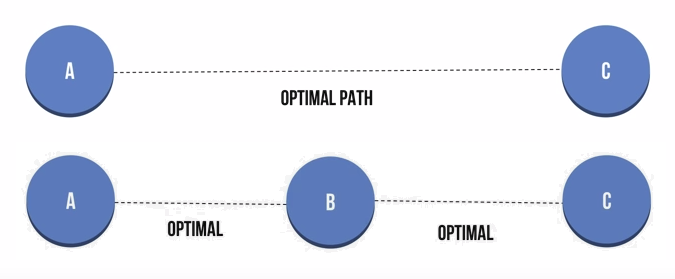
\includegraphics[width=\textwidth]{principle_of_optimality}
\caption{The principle of optimality shown for the case of finding optimal paths between points. The principle states, that we can find the optimal path from $A$ to $C$ (above) if we know the optimal paths from $A$ to $B$ and $B$ to $C$ (below).}
\label{fig:principle_of_optimality}
\end{figure}

This is also known as \textit{the principle of optimality}. Assume we have an optimal solution for the case $(A,C)$. Then that optimal solution should be obtainable from having the optimal solutions for the cases $(A,B)$ and $(B,C)$. Looking at figure \ref{fig:principle_of_optimality} where the principle is illustrated for the problem of finding optimal paths.

Since the principle can be applied iteratively, eventually the problem can be reduced to a set of "smallest", subsequent subproblems. Because of this, mathematical induction is often used to prove a given problem has optimal substructure.

\subsection{Overlapping subproblems}
This means that each of the subproblems occur "many times" and that we therefore can cache the solutions from these so we don't have to redo the same problem over and over.

\subsection{Example: Fibonacci numbers}
As is well known, the Fibonacci numbers are defined recursively:
\begin{equation}
F_0=0,\quad F_1=1,\quad F_{n+1}=F_n+F_{n-1} 
\end{equation}
By this very definition, it is clear that if we know the all $F_i, i\le n$ we can always find $F_{n+1}$, which means that the principle of optimality holds.

If we did this using only recursion, the fibonacci function would call itself a large number of times. We can prevent this by caching all $F_n$ that is calculated. Thus the overlapping subproblem criterion is also satisfied.

\section{The contraction mapping theorem}
Before we continue exploring dynamc programming in the context of reinforcement learning, let's take a mathematical side trek which will be convenient for showing the convergence of certain algorithms.

\begin{definition}
A contraction mapping on the metric space $(X,d)$ is a Lipschitz function $T: X\rightarrow X$ with Lipschitz constant $q\in[0,1[$, i.e.:
\begin{equation}
\forall x,y\in X:\ d(T(X),T(Y))\le q\cdot d(x,y)
\end{equation}
\end{definition}

\begin{theorem}
(The contraction mapping theorem) Let $T$ be a contraction mapping on the non-empty, complete metric space $(X,d)$. Then $T$ has a unique fixed-point $x^*$:
\begin{equation}
\exists !\ x^*\in X:\ T(x^*)=x^*
\end{equation}
This fixed-point can be found by iteration of $T$ from any starting point $x_0\in X$:
\begin{equation}
x_n=T(x_{n-1}),\quad (x_n)\underset{n\rightarrow\infty}{\rightarrow} x^*
\end{equation}
\end{theorem}
\begin{proof}
Using the triangle inequality for any $x,y\in X$ we have:
\begin{align}
d(x,y)&\le d(x,T(x)+d(T(x),T(y))+d(T(y),y)\\
&\le d(x,T(x)+q\cdot d(x,y)+d(T(y),y)
\end{align}
Here we've used that $T$ is a contraction. Isolate $d(x,y)$ to get:
\begin{equation}
d(x,y)(1-q)\le d(x,T(x)+d(T(y),y)\Leftrightarrow d(x,y)\le\frac{d(x,T(x)+d(T(y),y)}{1-q}
\label{fundamental_contraction_inequality}
\end{equation}
This is known as the \textit{fundamental contraction inequality}. We can use it to prove that $T$ has at most one fixed-point: Assume both $x$ and $y$ are fixed points. Then equation \ref{fundamental_contraction_inequality} says $d(x,y)\le 0$, leaving a distance of zero as the only option, which means that $x=y$.

Now, consider the mapping $T^n: X\rightarrow X$ defined as repeated application of $T$ $n$ times. This mapping is also a contraction, with Lipschitz constant $q^n$. We now wish to show that $(x_n)=(T^n(x_0))$ is Cauchy. We now apply the fundamental contraction inequality to $x_m$ and $x_n$:
\begin{align}
d(x_m,x_n)&\le\frac{d(x_m,T(x_m)+d(T(x_n),x_n)}{1-q}\\
&=\frac{d(T^m(x_0),T(T^m(x_0))+d(T(T^n(x_0)),T^n(x_0))}{1-q}\\
&=\frac{d(T^m(x_0),T^m(T(x_0))+d(T^n(T(x_0)),T^n(x_0))}{1-q}\\
&\le\frac{q^m\cdot d(x_0),T(x_0))+q^n\cdot d(T(x_0),x_0)}{1-q}\\
&=\frac{q^m+q^n}{1-q}d(x_0,T(x_0))
\end{align}
Since $q<1$, this can be made arbitrarily small by making $m$ and $n$ large enough. Hence $(x_n)$ is Cauchy and therefore convergent, since $X$ is complete. Let's call the limit $x^*$.

To show that $x^*$ is a fixed-point consider the recursive definition of the series:
\begin{equation}
x_{n+1}=T(x_n)
\end{equation}
Now apply the limit $n\rightarrow\infty$ on both sides of the equation:
\begin{equation}
\lim_{n\rightarrow\infty} x_{n+1}=\lim_{n\rightarrow\infty}T(x_n)
\end{equation}
Since $T$ is Lipschitz, it is also continuous, and so we may interchange limit and application of $T$:
\begin{equation}
\lim_{n\rightarrow\infty} x_{n+1}=T\left(\lim_{n\rightarrow\infty}x_n\right)
\end{equation}
But we know that both these limits are equal to $x^*$, so:
\begin{equation}
x^*=T(x^*)
\end{equation}
\end{proof}

The theorem is also known as \textit{Banach's fixed-point theorem}. By taking the limit $m\rightarrow\infty$ in the inequality in the proof, we get an estimate of the convergence speed towards $x^*$:
\begin{equation}
d(x^*,x_n)\le\frac{q^n}{1-q}d(x_0,T(x_0))
\end{equation}
So in each step of the iteration process, we get closer to the fixed-point at a factor of $q$ or lower.

\section{Dynamic programming for MDP's}
It turns out that we can use dynamical programming for finding value functions for MDP's. Here, the recursive substructure is implied by Bellman's optimality equations. And the value function can be cached as calculations are done. Hence, both criteria are satisfied.

This assumes perfect knowledge of the MDP, and therefore it can only be used for planning. There's essentially two types of question we can ask here:
\begin{itemize}
\item Prediction: Given a MDP $\langle\mathcal{S},\mathcal{A},\mathcal{P},\mathcal{R},\gamma\rangle$ and a policy $\pi$, what is the corresponding state-value function $v_\pi(s)$?
\item Control: Given a MDP $\langle\mathcal{S},\mathcal{A},\mathcal{P},\mathcal{R},\gamma\rangle$, what is the optimal state-value function $v_*(s)$?
\end{itemize}
We'll look at both below.

\subsection{Iterative policy evaluation}
Evaluation relies on prediction: Given a policy $\pi$ we want to find the state-value function $v_\pi(s)$. One approach - indeed the one we will use in this section - is to obtain the value function iteratively through Bellman's expectation equation \ref{expectation_state}. Here, we start by a guess $v_1$ - or simply zeros - at the state-value function as a vector, and then insert it into the expectation equation to get $v_2$. Iterating this process, getting $v_3, v_4, v_5$ etc., $v_n$ will eventually converge to $v_\pi$:
\begin{equation}
v_1\rightarrow v_2\rightarrow v_3\rightarrow\cdots\underset{n\rightarrow\infty}{\rightarrow}v_\pi
\end{equation}
We will prove this later.

The update is done using \textit{synchronous backup}, which means that we store the values of $v_i$ for all the states and use them to calculate the values for $v_{i+1}$. Only then are the "active" values used in the next step calculation changed.

\subsubsection{Example: Starting with $v_1=0$}
Assume out inital guess $v_1$ simply consists of all zeros. Then the second iteration is:
\begin{align}
v_2(s)=&\sum_{a\in\mathcal{A}}\pi(a|s)\left[\mathcal{R}^a_s+\gamma\sum_{s'\in\mathcal{S}}\mathcal{P}^a_{ss'}v_1(s')\right]=\\
&\sum_{a\in\mathcal{A}}\pi(a|s)\mathcal{R}^a_s
\end{align}
Similarly, the third iteration becomes:
\begin{align}
v_3(s)=&\sum_{a\in\mathcal{A}}\pi(a|s)\left[\mathcal{R}^a_s+\gamma\sum_{s'\in\mathcal{S}}\mathcal{P}^a_{ss'}v_2(s')\right]=\\
&\sum_{a\in\mathcal{A}}\pi(a|s)\left[\mathcal{R}^a_s+\gamma\sum_{s'\in\mathcal{S}}\mathcal{P}^a_{ss'}\sum_{a'\in\mathcal{A}}\pi(a'|s')\mathcal{R}^{a'}_{s'}\right]
\end{align}
And so on. Of course in practice this is done numerically.

\subsubsection{Example: Gridworld}

\begin{figure}
\centering
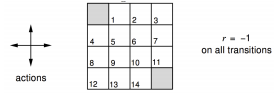
\includegraphics[width=0.6\textwidth]{gridworld}
\caption{The gridworld environment. The grey areas make up the terminal state.}
\label{fig:gridworld}
\end{figure}

Consider the gridworld environment shown in figure \ref{fig:gridworld}. The agent's state is the square it occupies. The possible action are moving up, down, left, or right. The grey squares make up a terminal state. Trying to move across the outer border will make the agent stay where it is. In each step before it reaches the terminal area, the reward is -1.

The policy $\pi$ we wish to examine is uniform random choice between the four available actions in any non-terminal state:
\begin{equation}
\pi(\uparrow|\cdot)=\pi(\rightarrow|\cdot)=\pi(\downarrow|\cdot)=\pi(\leftarrow|\cdot)=\frac{1}{4}
\end{equation}

\begin{figure}
\centering
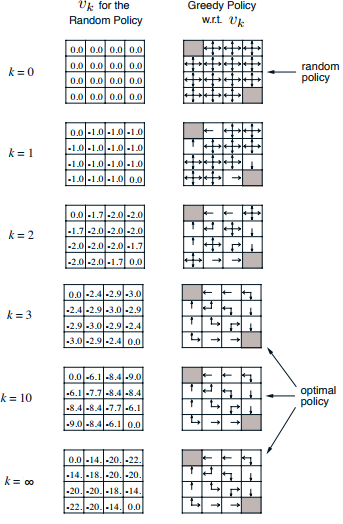
\includegraphics[width=0.9\textwidth]{iterative_policy_evaluation}
\caption{Left: Evolution of $v_k$ starting at zero. Right: The greedy policy corresponding to $v_k$.}
\label{fig:iterative_policy_evaluation}
\end{figure}

The left part of figure \ref{fig:iterative_policy_evaluation} shows how $v_k$ changes as the iterative policy evaluation process is performed. Eventually it converges; at $k=\infty$ the number at each square shows (save for the sign) the average number of steps a random walker takes before getting to the terminal state.

\subsection{Convergence of iterative policy evaluation}
So how are we sure that this iteration process actually converges? The answer has to do with the contraction mapping theorem.

Here, we consider each configuration of state-value function $v_n$ a point in euclidean space $X=\mathbb{R}^{|\mathcal{S}|}$ of dimension equal to the number of states. The distance we will use is the \textit{Manhattan distance}, or $d_\infty$ norm:
\begin{equation}
d(v,w)=\underset{s\in\mathcal{S}}{\max}|v(s)-w(s)|
\end{equation}
In each iteration step, the operator $T:X\rightarrow X$ is applied, here written in matrix form:
\begin{equation}
T: v\mapsto\mathcal{R}^\pi+\gamma\mathcal{P}v
\end{equation}
Given $v,w\in X$ we see:
\begin{align}
d(T(v),T(w))&=\underset{s\in\mathcal{S}}{\max}|\mathcal{R}^\pi+\gamma\mathcal{P}v-(\mathcal{R}^\pi+\gamma\mathcal{P}w)|\\
&=\underset{s\in\mathcal{S}}{\max}|\gamma\mathcal{P}v-\gamma\mathcal{P}w|\\
&=\gamma\cdot\underset{s\in\mathcal{S}}{\max}|\mathcal{P}(v-w)|\\
&\le\gamma\cdot d(v,w)
\end{align}
In the last step we used that none of the entries in $\mathcal{P}$ are larger than 1. So $T$ is a contraction with Lipschitz constant $q$ (assuming it is not exactly 1).

So by the contraction mapping theorem, the iterative process converges to a value of $v$ which is a fixed-point for $T$, i.e.:
\begin{equation}
T(v)=v\Leftrightarrow\mathcal{R}^\pi+\gamma\mathcal{P}v=v
\end{equation}
This is exactly the Bellman expectation equation, meaning the point of convergence is actually the state-value function for $\pi$.

\subsection{Control: Policy iteration}
Looking at the right hand side of figure \ref{fig:iterative_policy_evaluation}, we see the \textit{greedy policy} with respect to $v_k$. I.e. the policy that we choose the action for which the corresponding state is maximal (or if there's a tie, randomize even between those with maximal state-value).

These policies seem to be doing rather well. In fact, after only three iterations, it has arrived at the optimal policy, even if it takes way longer for $v_k$ to converge to $v_\pi$! This should give us an idea for how to improve our policy $\pi$:
\begin{enumerate}
\item Start with a policy $\pi$.
\item Find $v_\pi$ using iterative policy evaluation.
\item Construct the policy $\pi'=\textrm{greedy}(v_\pi)$.
\end{enumerate}
The new policy will always be better (or at least as good) as $\pi$:
\begin{equation}
\pi'\ge\pi
\end{equation}
We will show this in the next section. If the process is applied iteratively, it will always converge to an optial policy $\pi_*$. This is known as \textit{policy iteration}. Again, this will be shown in the next section.

For the gridworld example, only one such iteration was needed to reach an optimal policy. This is rarely the case for more complicated problems.

\subsection{Convergence of iterative policy improvement}
So why does all of this work? Let's start by considering only deterministic policies. Since greedy policies are deterministic (or can be made deterministic while retaining efficiency), this can be done without loss of generality.

So let $\pi$ be a deterministic policy, i.e.:
\begin{equation}
\pi(s)=a(s)
\end{equation}
Now make a new policy $\pi'$ by being greedy with respect to $v_\pi$. Recall, that according to Bellman's expectation equation:
\begin{equation}
v_\pi(s)=\sum_{a\in\mathcal{A}}\pi(a|s)q_\pi(s,a)=q_\pi(s,a(s))
\label{deterministic_policy}
\end{equation}
Here we have used that $\pi$ is deterministic. So being greedy corresponds to maximizing $q_\pi(a,s)$. This means:
\begin{equation}
\pi'(s)=\underset{a\in\mathcal{A}}{\textrm{argmax}}\ q_\pi(s,a)
\end{equation}
Why does this improve the policy? Let's see:
\begin{equation}
q_\pi(s,\pi'(s))=\underset{a\in\mathcal{A}}{\max}\ q_\pi(s,a)\ge q_\pi(s,a(s))=v_\pi(s)
\label{qv_inequality}
\end{equation}
In the last equal sign, we used equation \ref{deterministic_policy} again. Now we can use equation \ref{qv_inequality} and the definiton of $q_\pi$ to show the desired result:
\begin{equation}
v_\pi(s)\le q_\pi(s,\pi'(s))=\mathbb{E}_{\pi'}[R_t+\gamma v_\pi(S_{t+1})|S_t=s]
\end{equation}
Here we've used that the expectation value of a constant is simply the constant itself, meaning that $\gamma v_\pi(S_{t+1})=\mathbb{E}_{\pi'}[\gamma v_\pi(S_{t+1})]$. But now we may use \ref{qv_inequality} again:
\begin{equation}
v_\pi(s)\le\mathbb{E}_{\pi'}[R_t+\gamma q_\pi(S_{t+1},\pi'(s))|S_t=s]
\end{equation}
But now we can apply the same steps again to get:
\begin{equation}
v_\pi(s)\le\mathbb{E}_{\pi'}[R_t+\gamma R_{t+1}+\gamma^2 v_\pi(S_{t+2})|S_t=s]
\end{equation}
This can be iterated indefinitely, so in the end we get:
\begin{align}
v_\pi(s)\le&\mathbb{E}_{\pi'}[R_t+\gamma R_{t+1}+\gamma^2 R_{r+2}+\gamma^3 R_{r+3}+\cdots|S_t=s]=\\
&\mathbb{E}_{\pi'}[G_{t+1}|S_{t}=s]=v_{\pi'}(s)
\end{align}
This shows that $\pi\le\pi'$.

Now assume that we perform policy iteration until there is no further improvement. I.e. until:
\begin{equation}
v_\pi=v_{\pi'},\quad q_\pi=q_{\pi'}
\end{equation}
In this case, we can rewrite equation \ref{qv_inequality}, but this time with an equal sign:
\begin{equation}
q_\pi(s,\pi'(s))=\underset{a\in\mathcal{A}}{\max}\ q_\pi(s,a)=q_\pi(s,a(s))=v_\pi(s)
\end{equation}
But this means that $\pi$ satisfies the Bellman optimality equation:
\begin{equation}
v_\pi(s)=\underset{a\in\mathcal{A}}{\max}\ q_\pi(s,a)
\end{equation}
Hence $\pi$ is optimal. This shows convergence of iterative policy improvement.

\subsection{Modified policy iteration}
As we noticed in the gridworld example, sometimes we don't really need the full convergence of $v_*$ to get a good policy by acting greedy.

\textit{Modified policy iteration} exploits this idea by only taking $k$ steps in each policy evaluation loop.

\subsection{Value iteration}
This method explicity exploits the principle of optimality: An optimal strategy for an agent in state $s$ necesserily starts with a first optimal action $a_*$. If we know this, we can also choose the optimal action $a'_*$ in any state $s'$ the agent may end up in after taking action $a_*$. This is essentially what is expressed in Bellman's optimality equation:
\begin{equation}
v_*(s)=\underset{a}{\max}\left[\mathcal{R}^a_s+\gamma\sum_{s'\in\mathcal{S}}\mathcal{P}^a_{ss'}v_*(s')\right]
\end{equation}
Following the idea of iterative policy evaluation, we can start at some value of $v_*(s)$ and iterate this equation. This is known as \textit{value iteration}.

Since we're essentially being greedy in every update step, this is equivalent to modified policy iteration with $k=1$.

\subsubsection{Example: More gridworld}

\begin{figure}
\centering
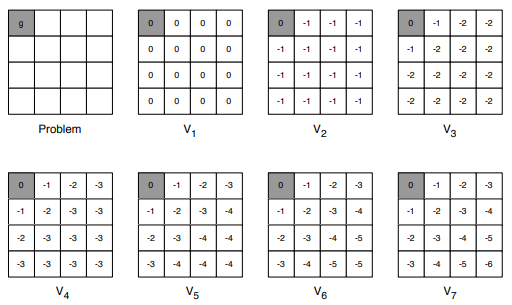
\includegraphics[width=0.9\textwidth]{value_iteration}
\caption{Left: Evolution of $v_k$ starting at zero. Right: The greedy policy corresponding to $v_k$.}
\label{fig:value_iteration}
\end{figure}

As an example, consider the gridworld from earlier, except with only one terminal square. The possible actions at each non-terminal square is still the four directions. But this time, we search for a value function instead of evaluating a policy. Figure \ref{fig:value_iteration} shows the state-value function as value iteration is performed starting from a uniform value of zero. We see that each step propagates the reward through the state space until convergence after 7 steps.

\section{Asynchronous dynamic programming}
So far, all the iterative processes have been synchronous. I.e. we've update all the states of the value functions at the same time. However, there's advantages to updating the values \textit{asynchronously}. The convergence will often become faster, and assuming all states are updated it is still guaranteed.

The rest of this section is a quick overview of three such strategies.

\subsection{In-place dynamic programming}
Here, one value at a time is updated as described above. The order in which the states are chosen is usually random, making sure all states are updated, and that no patterns affect the convergence process.

\subsection{Prioritised sweeping}
Not all states have the same impact on the convergence of the algorithms. As we saw in the gridword value iteration example in figure \ref{fig:value_iteration} change in value functions "ripple" out from certain states. The idea here, is the note how much the value changed in the previous update. Then sort them based on the absolute value of the change and do the updates in this order. A state that has changed a lot tends to have more effect on subsequent updates, so with this approach, we should get more change in values overall.

This can be implemented using a priority queue data sctructure.

\subsection{Real-time dynamic programming}
Here, we focus on updating the states that are most relevant for the agent. This is done by simulating an agent moving through the state space, and then only updating states it comes into contact with.

\section{Model-free prediction}
So far we have focused on planning. In other words, the situation where er know all the details of the environment. Obviously, this is not alwys the case.

In this section we will consider the predicion problem in the case of an MDP we don't know the details of. This is known as \textit{model-free prediction}.

\subsection{Monte Carlo learning}
To use what is known as the \textit{Monte Carlo (MC) learning} method, we must have a process which terminates at some point - the method only learns from what is known as \textit{full episodes}.

So given a policy $\pi$, we can start an agent in state $S_1\in\mathcal{S}$ and then let the process run, following $\pi$, getting rewards and so on, until the episode terminates at step $k$. The total episode can then be summed up as:
\begin{equation}
S_1, A_1, R_1, S_2, A_2, R_3,\ldots,S_k
\end{equation}
At any step in the episode $t$, we can then calculate the discounted reward:
\begin{equation}
G_t=R_{t+1}+\gamma R_{t+2}+\gamma^2 R_{t+3}+\gamma^{k-t-1}R_{k-1}
\end{equation}
Recall that the state-value function is the expected value of this:
\begin{equation}
v_\pi(s)=\mathbb{E}_\pi[G_t|S_t=s]
\end{equation}
According to the law of large numbers, if we take the average of a large number of actualized values, we will converge to the expected value with probability 1. In other words, if we run this a lot of times $n\gg 1$, each time starting in state $S_1=s$ and getting discounted reward $G^i_1$ (i.e. calculated from step 1) in the $i$'th run, we have:
\begin{equation}
v_\pi(s)\approx\frac{1}{n}\sum_{i=1}^n G^i_1
\end{equation}
Now, of course, we need not start at position $s$. If we end up at $s$ at any time during the episode, we can n different approaches.

\subsubsection{First-visit MC evaluation}
Here, to estimate $v_\pi(s)$ from a set of $n$ episodes (with random starting states), we count how many episodes $s$ is reached $N(s)$. For each such episode, we calculate the discounted reward from the $first visit$ to $s$ in the episode $G^j_{\textrm{first}}$. We may now estimate the state-value function as:
\begin{equation}
v_\pi(s)\approx\frac{1}{N(s)}\sum_{j=1}^{N(s)} G^j_{\textrm{first}}
\end{equation}

\subsubsection{Every-visit MC evaluation}
But of course, because of the Markov property, there's not fundamental difference between the first time we visit state $s$ in an episode, from any subsequent times. In other words, we might as well include all the times $s$ is visited in any episode. That total number of visits plays the part of $N(s)$ here. The discounted reward is calculated from each of these $G^j_{t_j}$. The formula for the approximate state-value function is then:
\begin{equation}
v_\pi(s)\approx\frac{1}{N(s)}\sum_{j=1}^{N(s)} G^j_{t_j}
\end{equation}

\subsection{Incremental mean}
In either of the two cases above, instead of waiting until we've found all the relevant visits and then averaging, we might as well have done a running calculation of the mean.

To see how this works, consider a sequence of observations $x_1,x_2,\ldots$. For the $k$'th step, we may calculate the mean for the first $k$ values:
\begin{equation}
\mu_k=\frac{1}{k}\sum_{i=1}^k x_i
\label{mean}
\end{equation}
Our goal is to calculate $\mu_k$ just from $\mu_{k-1}$ and $x_k$. Rewrite equation \ref{mean} as follows:
\begin{align}
\mu_k&=\frac{1}{k}\left(\sum_{i=1}^{k-1}x_i+x_k\right)\\
&=\frac{1}{k}((k-1)\mu_{k-1}+x_k)\\
&=\mu_{k-1}+\frac{1}{k}(x_k-\mu_{k-1})
\end{align}
One way to think of this, is that $\mu_{k-1}$ is the best estimate so far. $x_k-\mu_{k-1}$ is how much the new observation is off, and so we adjust $\mu_k$ to fit it.

\subsubsection{Incremental mean for Monte Carlo method}
Here, when we get to the $k$'th (first if first-visit) visit to state $s$, with a discounted reward $G_k$, the update can be written:
\begin{equation}
v_\pi(s)\approx V_k(s)=V_{k-1}(s)+\frac{1}{k}(G_k-V_{k-1}(s))
\end{equation}
Here, we use the notation of $V_k(s)$ for the guess after the $k'th$ observation.

\subsubsection{Incremental mean for non-stationary processes}
As we can see, we continually need to keep track of how many measurements we have done so far to use incremental means. However, if the process is \textit{non-stationary}, i.e. if it eventually changes over time, we don't really want to consider episodes that are too far in the past. In this case, we may alter the incremental mean formula to:
\begin{equation}
v_\pi(s)\approx V_k(s)=V_{k-1}(s)+\alpha(G_k-V_{k-1}(s))
\label{incremental_nonstationary}
\end{equation}
Here we don't need to keep track of $k$. Instead, we essentially assume, that only the last $1/\alpha$ visits are important.

\subsection{Temporal-difference learning}
\textit{Temporal-difference (TD) learning} is another model-free policy evaluation method. However, in contrast to MC, TD can learn from \textit{incomplete episodes}. This has the advantage that the process need not always terminate. This is done by what is known as \textit{bootstrapping}.

\subsection{TD(0)}
If we look at equation \ref{incremental_nonstationary}, we can interpret is as follows:
\begin{equation}
\textrm{new value}=\textrm{old value}+\alpha(\textrm{estimated reward}-\textrm{old value})
\end{equation}
Previously, we've estimated the future discounted reward by actually calculating it from the terminating episode. But we could also estimate it is:
\begin{equation}
\textrm{immediate reward}+\gamma\cdot\textrm{future reward}
\end{equation}
For the future reward, our best guess is the currently estimated value. So, in other words, this gives us the following update rule for our estimate:
\begin{equation}
V(S_t)\mapsto V(S_t)+\alpha(R_{t+1}+\gamma V(S_{t+1})-V(S_t)) 
\end{equation}
This method is known as \textit{TD(0)}. We will make the following two definitions:
\begin{itemize}
\item $R_{t+1}+\gamma V(S_{t+1})$ is known as the \textit{TD target}.
\item $\delta_t=R_{t+1}+\gamma V(S_{t+1})-V(S_t)$ is called the \textit{TD error}.
\end{itemize}

\subsection{Bias-variance tradeoff}
Let's consider the properties of the MC vs. TD(0) learning estimates.

For MC learning we consider many time steps - whole episodes. Since this is an ordinary average, the estimate is unbiased. However, we will have a tendency to overfit to the actually observed episodes, exactly since we're considering long stretches of time. To see why: Consider an agent which goes through an episode and eventually "dies" (terminates). If this was a human, and we're trying to estimate the cause of death, it is possible that recent events (not looking both ways before crossing the road) was the cause of death, as opposed to things that happened long time ago (a food poisoning 3 years ago). Since everything is considered, the algorithm will often find patterns where there are none. In other words, it will overfit, i.e. have a high variance. But since everything is considered, given enough data, eventually it will find the true causes - it is unbiased.

On the other hand, for TD learning, we only consider the very recent actions/rewards in each step. In the analogy above, this means that we are more likely to identify immediate causes/rewards. Long term patterns are very hard to find, but on the other hand, it doesn't see patterns where there are none. So the algorithm has a high bias, but low variance.

Another view is that MC is based on a lot of sample points, which means that there's a lot of aggregated noise, but on the other hand, having many points will make sure we're close to the real value. For TD, the situation is reversed: Only one point is used, meaning that there's only noise from one point, but it is also hard to estimate true value.

Luckily, it turns out that there is a way to choose an algoritm that is a compromise between these two extremes, which allows us to tune the bias-variance tradeoff to suit our needs.

\subsection{$n$-step temporal-difference learning}
So far, the temporal difference has only been one step into the future. But there's nothing preventing us from us looking more than one step ahead in our estimates, changing the TD target as appropriate. We can look $n$ steps ahead:
\begin{align}
G^{(1)}(t)=&R_{t+1}+\gamma V(S_{t+2})\\
G^{(2)}(t)=&R_{t+1}+\gamma R_{t+2}+\gamma^2 V(S_{t+2})\\
\vdots\quad & \quad\vdots\\
G^{(\infty)}(t)=&R_{t+1}+\gamma R_{t+2}+\gamma^2 R_{t+3}+\dots
\end{align}
Notice that the limiting case is the same as Monte Carlo learning, as all subsequent steps are taken into account. 

So the update rule for $n$-step temporal-difference learning becomes:
\begin{equation}
V(S_t)\mapsto V(S_t)-\alpha(G^{(n)}-V(S_t))
\end{equation}
This is very similar to the gradient descent algorithm for training neural networks. Here, $\alpha$ plays the part of the learning rate, while the parenthesis can be thought of as an error (similar to a derivative).

\subsection{TD($\lambda$)}
So $n=1$ and $n=\infty$ are two extremes corresponding to TD(0) and MC respectively. Meaning that low $n$ has high bias, low variance. And high $n$ has low bias, high variance. It turns out that there is a better way of tuning the tradeoff, though.

Instead of using simply one $n$, a sum over all values of $n$ is used. This is done by using a weight $\lambda\in[0,1]$. The target is then set to:
\begin{equation}
G^\lambda_t=(1-\lambda)\sum_{n=1}^\infty\lambda^{n-1}G^{(n)}_t
\end{equation}
This known as the $\lambda$-\textit{return}. The weights add up to 1, because of the geometric series:
\begin{equation}
\sum_{n=0}^\infty\lambda^n=\frac{1}{1-\lambda}
\end{equation}
Hence $1-\lambda$ acts as a normalization constant. If the episode terminates, we assign the remaining weight to the highest possible value of $n$.

We see that when $\lambda=0$ we do indeed get TD(0). When $\lambda=1$, and the episode terminates, all but the last weight is zero, and we get MC.

\subsection{Overview of RL algorithms}
Let's pause for a moment and consider the strategies of the algorithms we've seen so far.

\begin{figure}
\centering
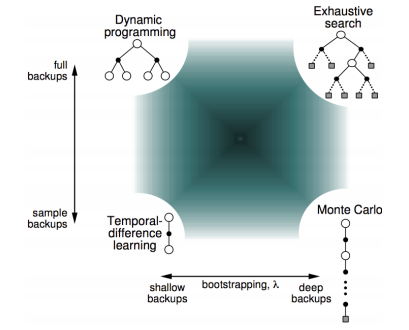
\includegraphics[width=\textwidth]{rl_overview}
\caption{Backup space for algorithms.}
\label{fig:rl_overview}
\end{figure}

\subsubsection{Backup}
Figures \ref{fig:rl_overview} and \ref{fig:backups} show different approaches to the \textit{backup} strategy used so far. The first axis in figure \ref{fig:rl_overview} shows the \textit{depth} of the backup, while the second axis shows the \textit{width} of the backup.

Consider first the brute force approach of an exhaustive search. Here all of the data are used - not merely samples - which means that the backup is \textit{full}. In every step of iteration, the entire path back to the starting point is used, which means that the backup is \textit{deep}.

Dynamic programming still uses full backups - all data are used. But here, in each step, the backup is \textit{shallow}, as we only look one step forward in the data.

Monto Carlo learning is based on a sample, and hence uses \textit{sample} backup. But it uses the data for all of the episode, so the backup is also deep.

TD(0) learning uses sample backup as well. But since we only look one step ahead, the backup is shallow.

Finally, TD($\lambda$) learning uses sample backups too. But it allows us to move along the first axis, from shallow to deep backup as $\lambda$ varies.

\begin{figure}
\centering
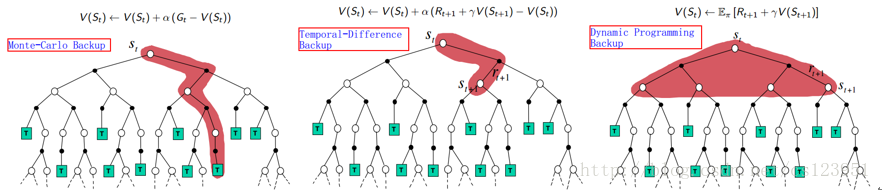
\includegraphics[width=\textwidth]{backups}
\caption{Illustration of backups for MC, TD(0), and DP respectively. An exhaustive search would cover all of the tree.}
\label{fig:backups}
\end{figure}

\subsubsection{Bootstrapping and sampling}
In statistics, a \textit{bootstrap} is the process of resampling data. In RL, an algorithm is said to use bootstrapping, if the update involves an estimation based on previous prediction.

Dynamic programming bootstraps, as seen from the Bellman equation. Temporal difference learning bootstraps as well. Monte Carlo learning does not, as it is instead based on the entire episode sample.

An algorithm that does not involve an expectation value, i.e. an estimate including all possible future outcomes is said to \textit{sample}. Monte Carlo and TD samples, while dynamic programming does not.

\subsubsection{Online vs. offline learning}
An algorithm can be operate \textit{online} or \textit{offline}. In this context it depends on when the updates to the value functions are done. Online learning means that values are changed while the episode still runs - it is done after every single action. Offline learning, on the other hand is done after the entire episode is finished.

\subsection{Backward view: Eligibility traces}
So far we have been taking a \textit{forward view}, looking $n$ steps forward into the process and so on. However, in practice, we want to do updates based on what went before our current time step. To do so, we use the tool of \textit{eligibility traces} for TD($\lambda$):

At time step zero, we set the \textit{eligibilty} $E$ of all states equal to zero: $E_0(s)=0$. These are then updated in each time step according to the following rules:
\begin{itemize}
\item All eligibilities are reduced as follows: $E_t(s)=\lambda\gamma E_{t-1}(s)$
\item If $S_t=s$, then in addition to the discounting above, 1 is added to eligibility. So all in all: $E_t(s)=\lambda\gamma E_{t-1}(s)+1$
\end{itemize}
After this, $V(s)$ is updated for all $s$, so that the change is proprotional to $E_t(s)$ and the SD error $\delta_t$:
\begin{equation}
\delta_t=R_{t+1}+\gamma V(S_{t+1})-V(S_t)
\label{delta_def}
\end{equation}
Update rule (for all $s$) is:
\begin{equation}
V(s)\mapsto V(s)-\alpha\delta_t E_t(s)
\end{equation}

\subsection{Equivalence between views}
It turns out that the forward and backward views are equivalent, at least for offline learning, i.e. when the updates are only done once the episode is over.

\begin{theorem}
The sum of offline updates for state $s$ is the same for forward and backward views in TD($\lambda$):
\begin{equation}
\sum_{t=1}^{T-1}\alpha\left(G^{(\lambda)}_t-V(S_t)\right)\cdot 1_{S_t=s}=\sum_{t=1}^{T-1}\alpha\delta_t E_t(s)
\end{equation}
Here $1_{S_t=s}$ is equal to 1 when $S_t=s$, and 0 otherwise.
\end{theorem}

\begin{proof}
Let's start by the special cases of the extreme values of $\lambda$.

When $\lambda=0$, the eligibility traces are all reset each step. Which means that for a time step $t$ where $S_t=s$, $E_t(s)=1$, and otherwise all elegibility traces are zero. This is exactly equivalent to (offline) TD(0) learning.

On the other hand, if $\lambda=1$, the eligibility traces decay only according to $\gamma$. This means that the eligibilty trace for a state $E_t(s)$ keeps track of how many times the state $s$ has been visited up to and including time $t$. First, let's consider the case where $s$ is visited once, at time step $k$. This means that the eligibility function is:
\begin{equation}
E_t(s)=\begin{cases}
0 & \textrm{for }t<k \\
\gamma^{t-k} & \textrm{for }t\ge k
\end{cases}
\end{equation}
This means that the right hand sum is:
\begin{equation}
\sum_{t=1}^{T-1}\alpha\delta_t E_t(s)=\alpha\sum_{t=k}^{T-1}\gamma^{t-k}\delta_t
\end{equation}
Using the definition in equation \ref{delta_def} this is:
\begin{equation}
\alpha\sum_{t=k}^{T-1}\gamma^{t-k}\left[R_{t+1}+\gamma V(S_{t+1})-V(S_t)\right]
\end{equation}
Writing out each term in the sum:
\begin{align}
&R_{k+1}+\gamma V(S_{k+1})-V(S_k)\\
+&\gamma R_{k+2}+\gamma^2 V(S_{k+2})-\gamma V(S_{k+1})\\
+&\gamma^2 R_{k+3}+\gamma^3 V(S_{k+3})-\gamma^2 V(S_{k+2})\\
+&\cdots\\
+&\gamma^{T-1-k} R_T+\gamma^{T-k}V(S_T)-\gamma^{T-1-k} V(S_{T-1})
\end{align}
A lot of terms now cancel leaving
\begin{equation}
R_{k+1}+\gamma R_{k+2}+\gamma^2 R_{k+3}+\cdots +\gamma^{T-1-k}R_T-V(S_k)=G^{(1)}_k-V(S_k)=\delta_k
\end{equation}
Here we've also used that $V(S_T)=0$ since the state is terminal. So in the case where $s$ is visited once, we get (first-visit) Monte Carlo learning result. If $s$ is revisited, there's wil be a contribution for each visit. But since elegibility traces are additive with respect to several visits, the equality remains true.

The general case is very similar to the $\lambda=1$ calculation. Again, assume that $s$ is visited once, at time $k$. Now, the eligibility trace is:
\begin{equation}
E_t(s)=\begin{cases}
0 & \textrm{for }t<k \\
(\lambda\gamma)^{t-k} & \textrm{for }t\ge k
\end{cases}
\end{equation}
The right hand sum now becomes:
\begin{equation}
\alpha\sum_{t=k}^\infty(\lambda\gamma)^{t-k}\left[R_{t+1}+\gamma V(S_{t+1})-V(S_t)\right]
\end{equation}
Since the episode is no longer required to terminate, we can sum to infinity here. Write out the sum, and move terms to make time steps line up:
\begin{align}
-V(S_k)+&R_{k+1}+\gamma V(S_{k+1})-\lambda\gamma V(S_{k+1})\\
+&\lambda\gamma\left[R_{k+2}+\gamma V(S_{k+2})-\lambda\gamma V(S_{k+2})\right]\\
+&(\lambda\gamma)^2\left[R_{k+3}+\gamma V(S_{k+3})-\lambda\gamma V(S_{k+3})\right]\cdots
\end{align}
Pull out factors of $1-\lambda$:
\begin{align}
-V(S_k)+&R_{k+1}+\gamma(1-\lambda)V(S_{k+1})\\
+&\lambda\gamma\left[R_{k+2}+\gamma(1-\lambda)V(S_{k+2})\right]\\
+&(\lambda\gamma)^2\left[R_{k+3}+\gamma(1-\lambda)V(S_{k+3})\right]+\cdots
\end{align}
Now remember that:
\begin{equation}
\sum_{n=0}^\infty\lambda^n=\frac{1}{1-\lambda}
\end{equation}
Use this to rewrite:
\begin{equation}
R_t=(1-\lambda)\frac{R_t}{1-\lambda}=(1-\lambda)\sum_{n=0}^\infty R_t\lambda^n
\end{equation}
So we can also pull out factors of $1-\lambda$ from the rewards, so that we get (here is sum notation):
\begin{equation}
(1-\lambda)\left[\sum_{m=0}^\infty(\lambda\gamma)^m\left(\sum_{n=0}^\infty R_{k+m}\lambda^n+\gamma V(S_{k+m+1})\right)\right]-V(S_k)
\end{equation}
We now wish to group the contents of the parenthesis by powers of $\lambda$. If we want all terms of power $p$, then we must have $p=m+n$. Or $m=p-n$. Remembering that $m\ge 0$, this means:
\begin{equation}
(1-\lambda)\sum_{p=0}^\infty\lambda^p\left[\sum_{n\le p}^\infty \gamma^n R_{k+p-n}+\gamma^{p+1}V(S_{k+p-n+1})\right]-V(S_k)
\end{equation}
On closer inspection, this is:
\begin{equation}
G^\lambda_k-V(S_k)
\end{equation}
For more than one visit to $s=S_k$, this generalizes as above.
\end{proof}

\begin{figure}
\centering
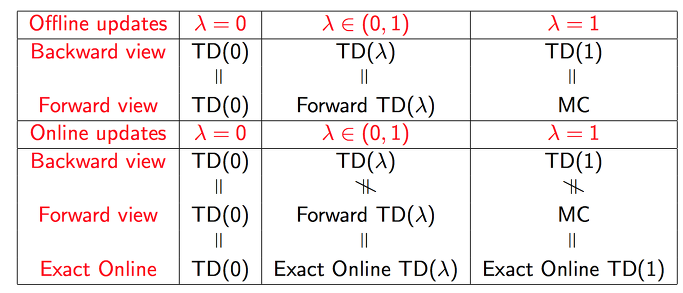
\includegraphics[width=\textwidth]{offline_online}
\caption{Comparison of forward/backward views and offline/online updates for TD learning.}
\label{fig:offline_online}
\end{figure}

\section{Model-free control}
Last section dealt with evaluating a policy, but usually what we really want it control - finding an optimal policy. Again, we will take a model-free approach. This is useful, because even if the underlying model is a MDP, we may not know it. Or we may know it, but it's too big to handle without sampling.

\subsection{On- and off-policy learning}
We may learn about policy $\pi$ by actually following the policy $\pi$ (when doing control, we want to improve it along the way). This is known as \textit{on-policy} learning. But we may also learn about $\pi$ by following another policy $\mu$ - "looking over the shoulder" of it, so to speak.

At first we will focus on on-policy learning.

\subsection{Generalized policy iteration}
We want to mimic the strategy of policy iteration, generalizing it to the model-free case. Recall that policy iteration consists of two components:
\begin{itemize}
\item Policy evauation: We can use - say MC learning - to estimate $v_\pi$ for the current policy $\pi$.
\item Policy improvement: Improve the model by acting greedily with respect to $v_\pi$.
\end{itemize}
Each of these components are problematic in the model free case:
\begin{itemize}
\item Policy evaluation of $v_\pi$ requires knowledge of the underlying MDP model.
\item When we're acting greedily, we may cut off parts of the state space which has a long-time reward payoff.
\end{itemize}

 

\end{document} 
